
\section{Resonance sea state }

Dynamic sea state resonance shall be analysed especially for low frequent wind turbine configurations. The identification of the sea state that creates highest excitation loads can be performed in two ways.\\
a) Dynamic fatigue loads are proportional to $\sqrt{S_{\zeta \zeta}\left(\omega_{0}\right)}$, where $S_{\zeta \zeta\left(\omega_{0}\right)}$ is the spectral energy of the wave spectrum at first eigenfrequency Fehler! Verweisquelle konnte nicht gefunden werden.. This can be derived from frequency domain calculations for a narrow band response, which is a good approximation in case dynamic excitation is significant. It is denoted as Resonant Wave Intensity (RWI).\\

\begin{figure}[H] 
 \centering 
 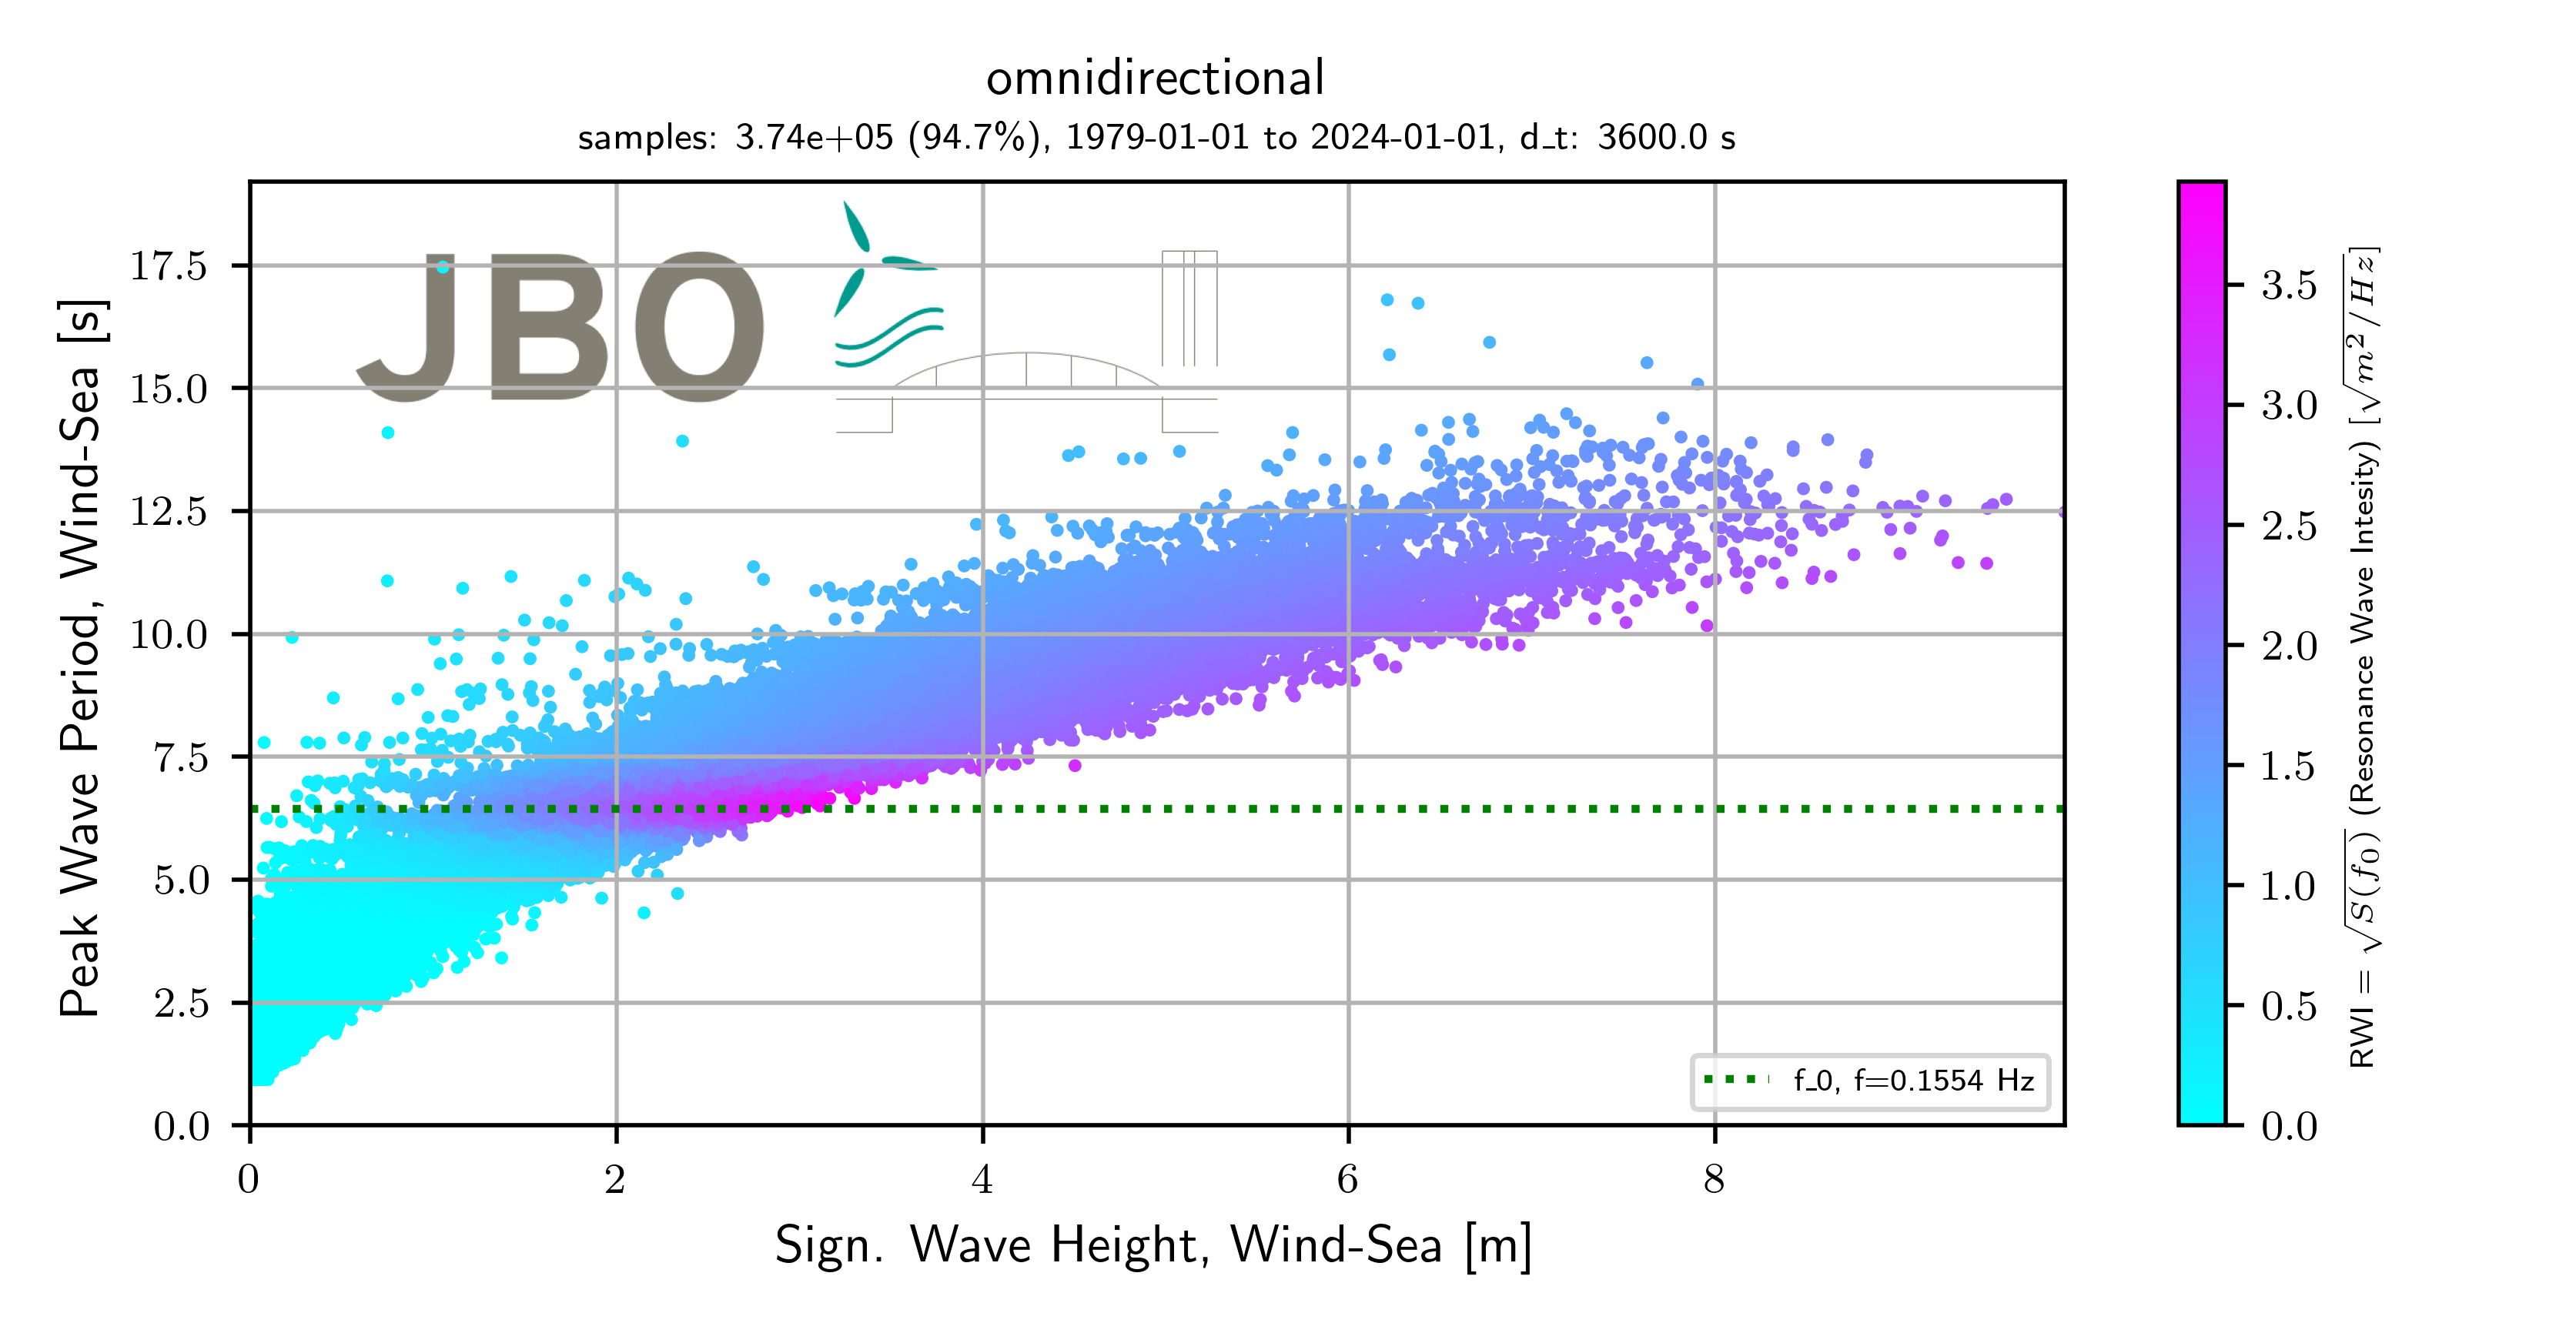
\includegraphics[width=1.0\textwidth]{C:/Users/aaron.lange/Desktop/Projekte/Hindcast_Tool/HindTool/example_output/RWI_wind_page_3.png} 
 \caption{ RWI-wind-page-3 } 
 \label{fig: RWI_wind_page_3 } 
\end{figure}
b) Assessment of frequency domain DEL of the bending moment at mudline for idling conditions using modal superposition.\\

\begin{figure}[H] 
 \centering 
 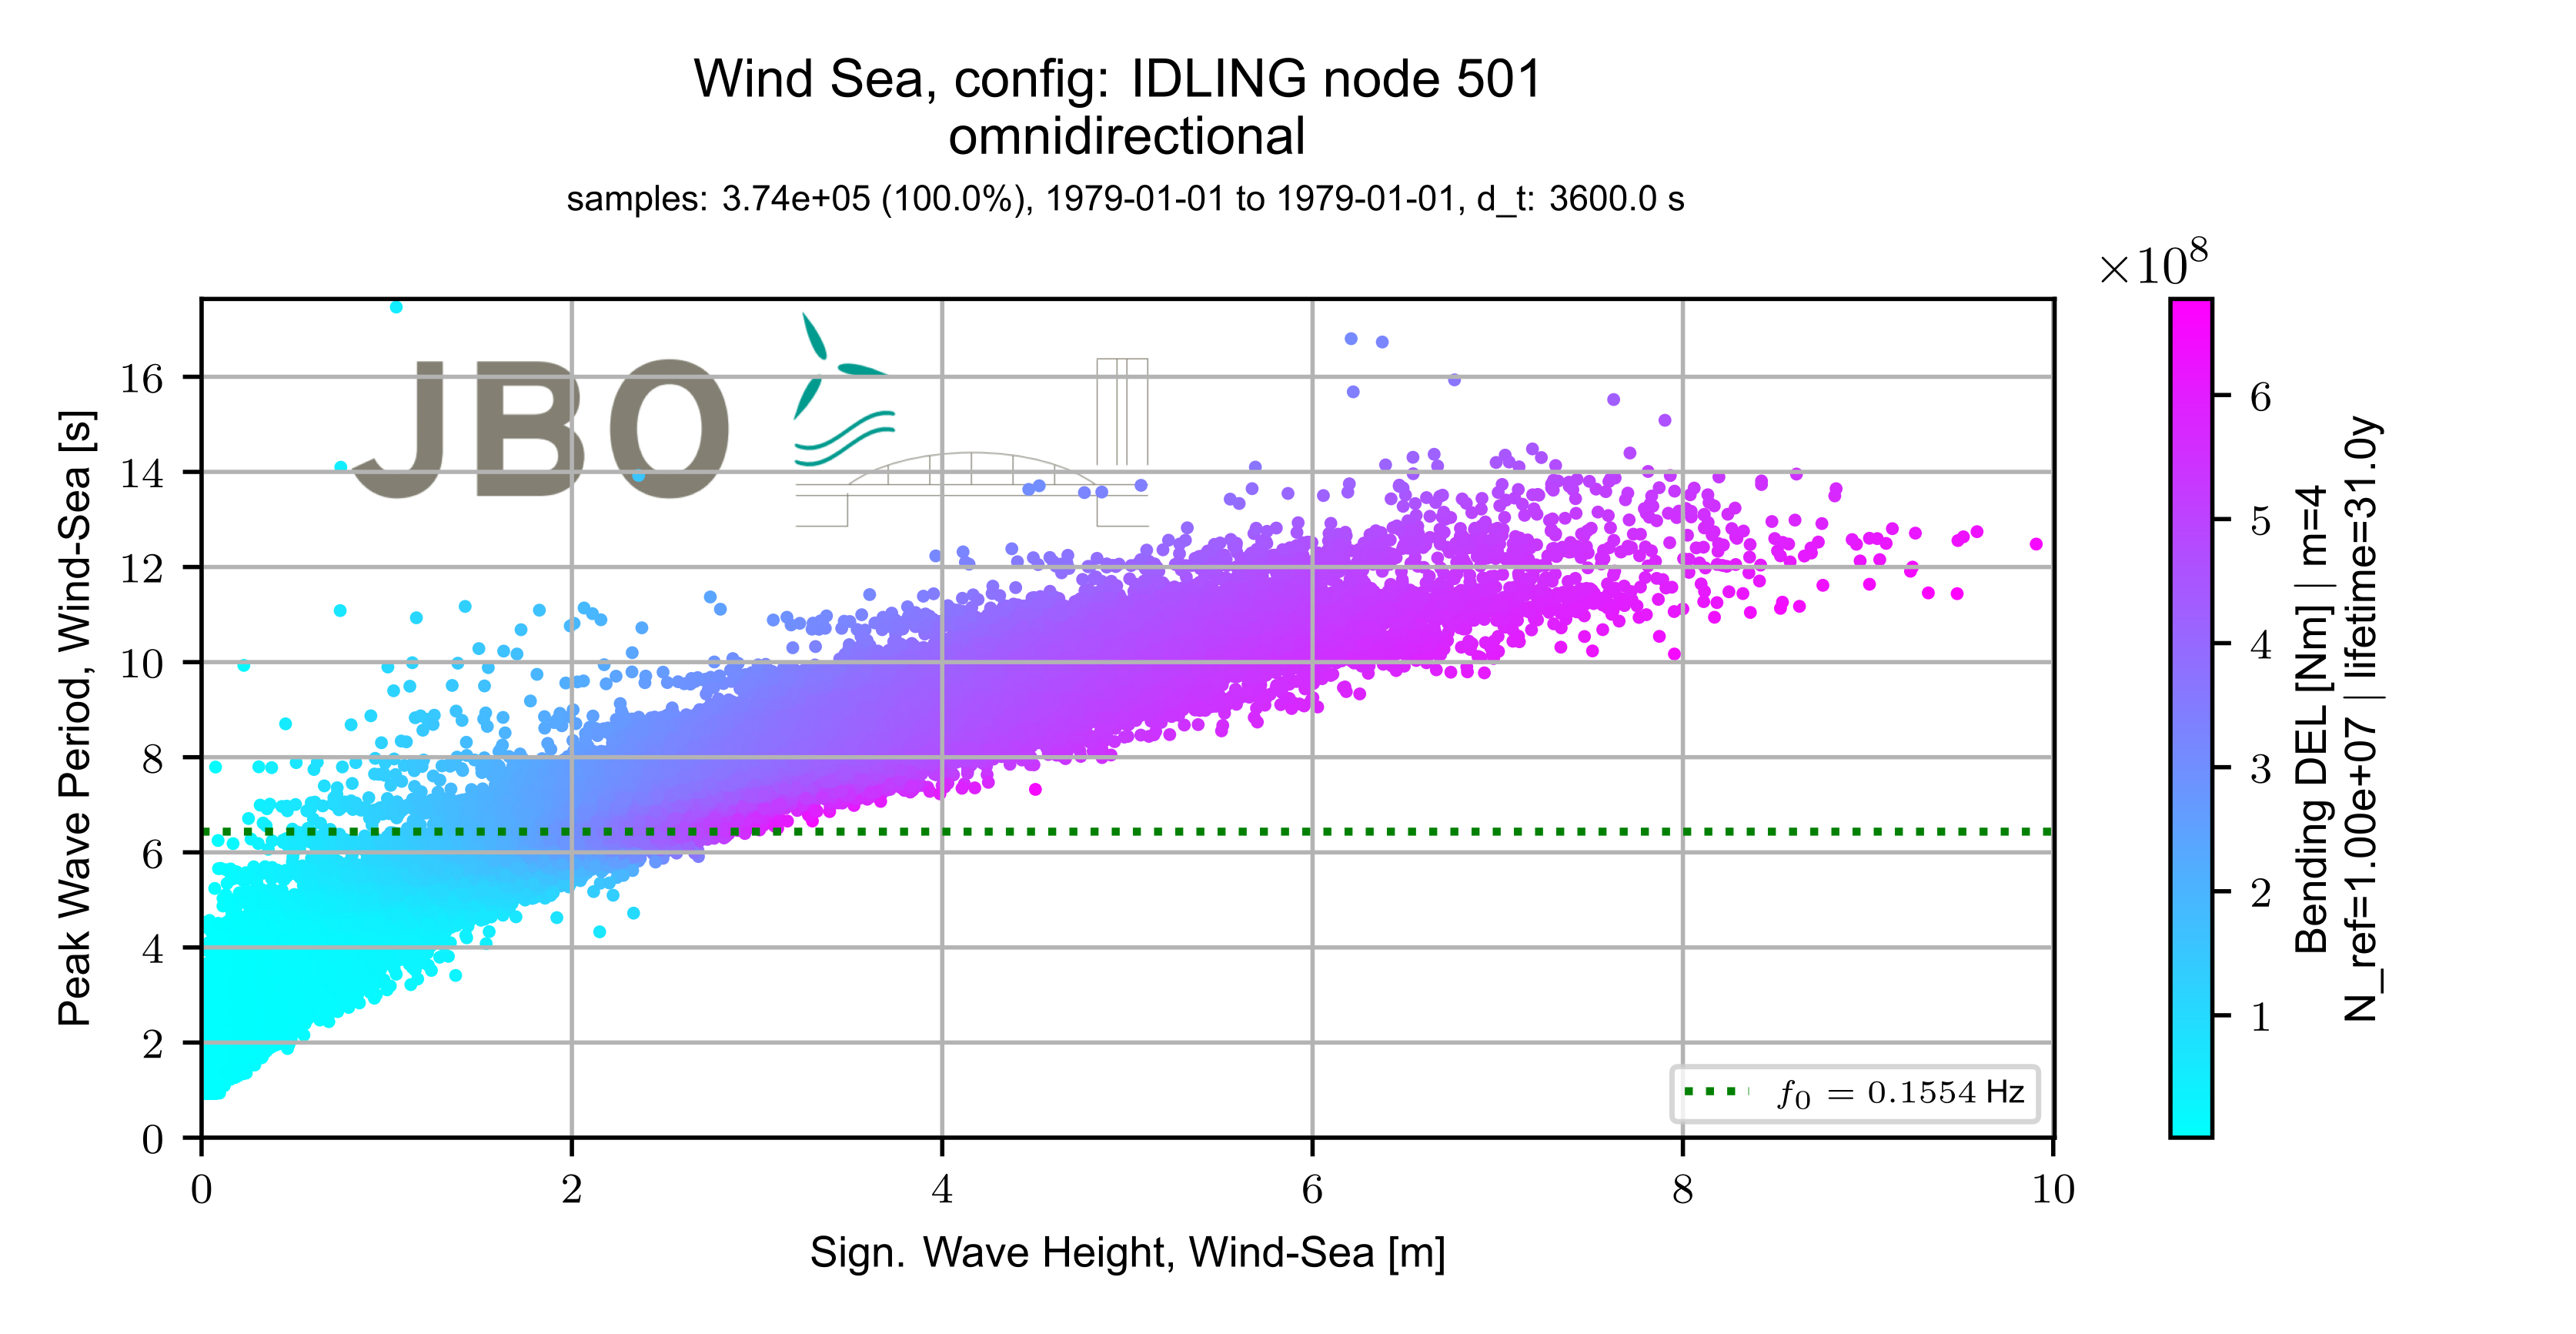
\includegraphics[width=1.0\textwidth]{C:/Users/aaron.lange/Desktop/Projekte/Hindcast_Tool/HindTool/example_output/Valid_scatter_wind_page_3.png} 
 \caption{ Valid-scatter-wind-page-3 } 
 \label{fig: Valid_scatter_wind_page_3 } 
\end{figure}

A comparison of the most Severe Seastates is shown in table REF. ERKLÄRUNG BEI ABWEICHUNG??
\begin{figure}[H] 
 \centering 
 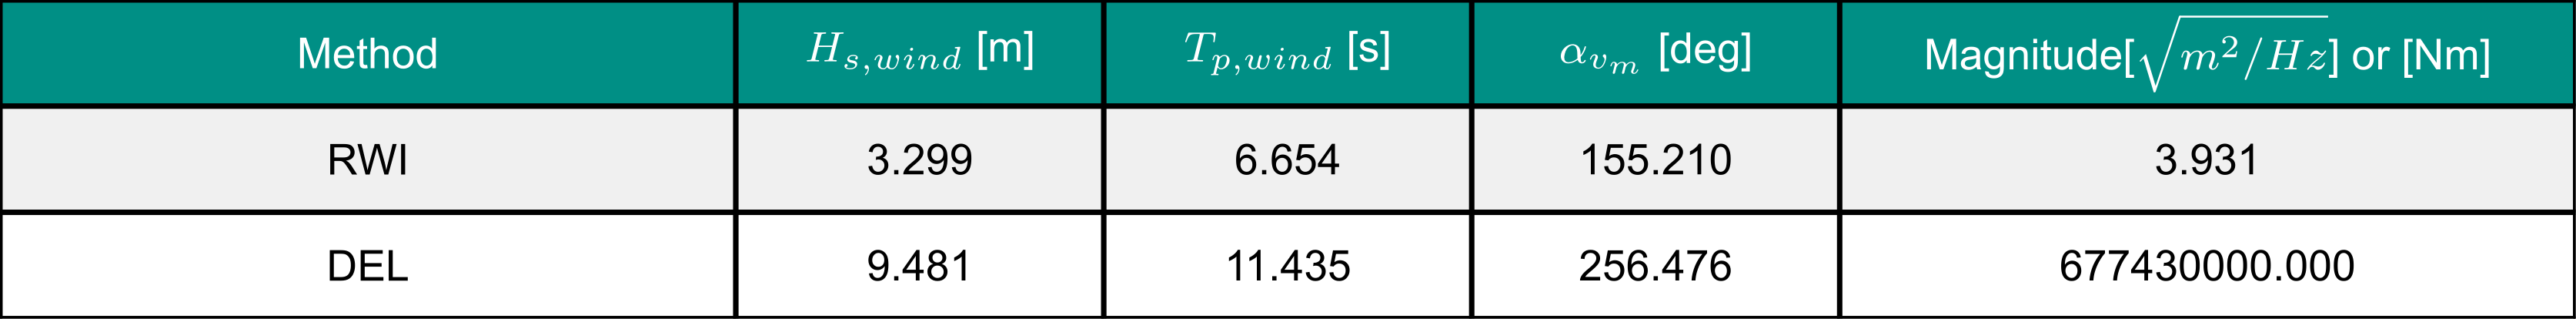
\includegraphics[width=1.0\textwidth ]{C:/Users/aaron.lange/Desktop/Projekte/Hindcast_Tool/HindTool/example_output/Resonance_compare_page_1.png} 
 \captionsetup{type=table} 
\caption{ Resonance-compare-page-1 } 
 \label{tab: Resonance_compare_page_1 } 
\end{figure}

\begin{figure}[H] 
 \centering 
 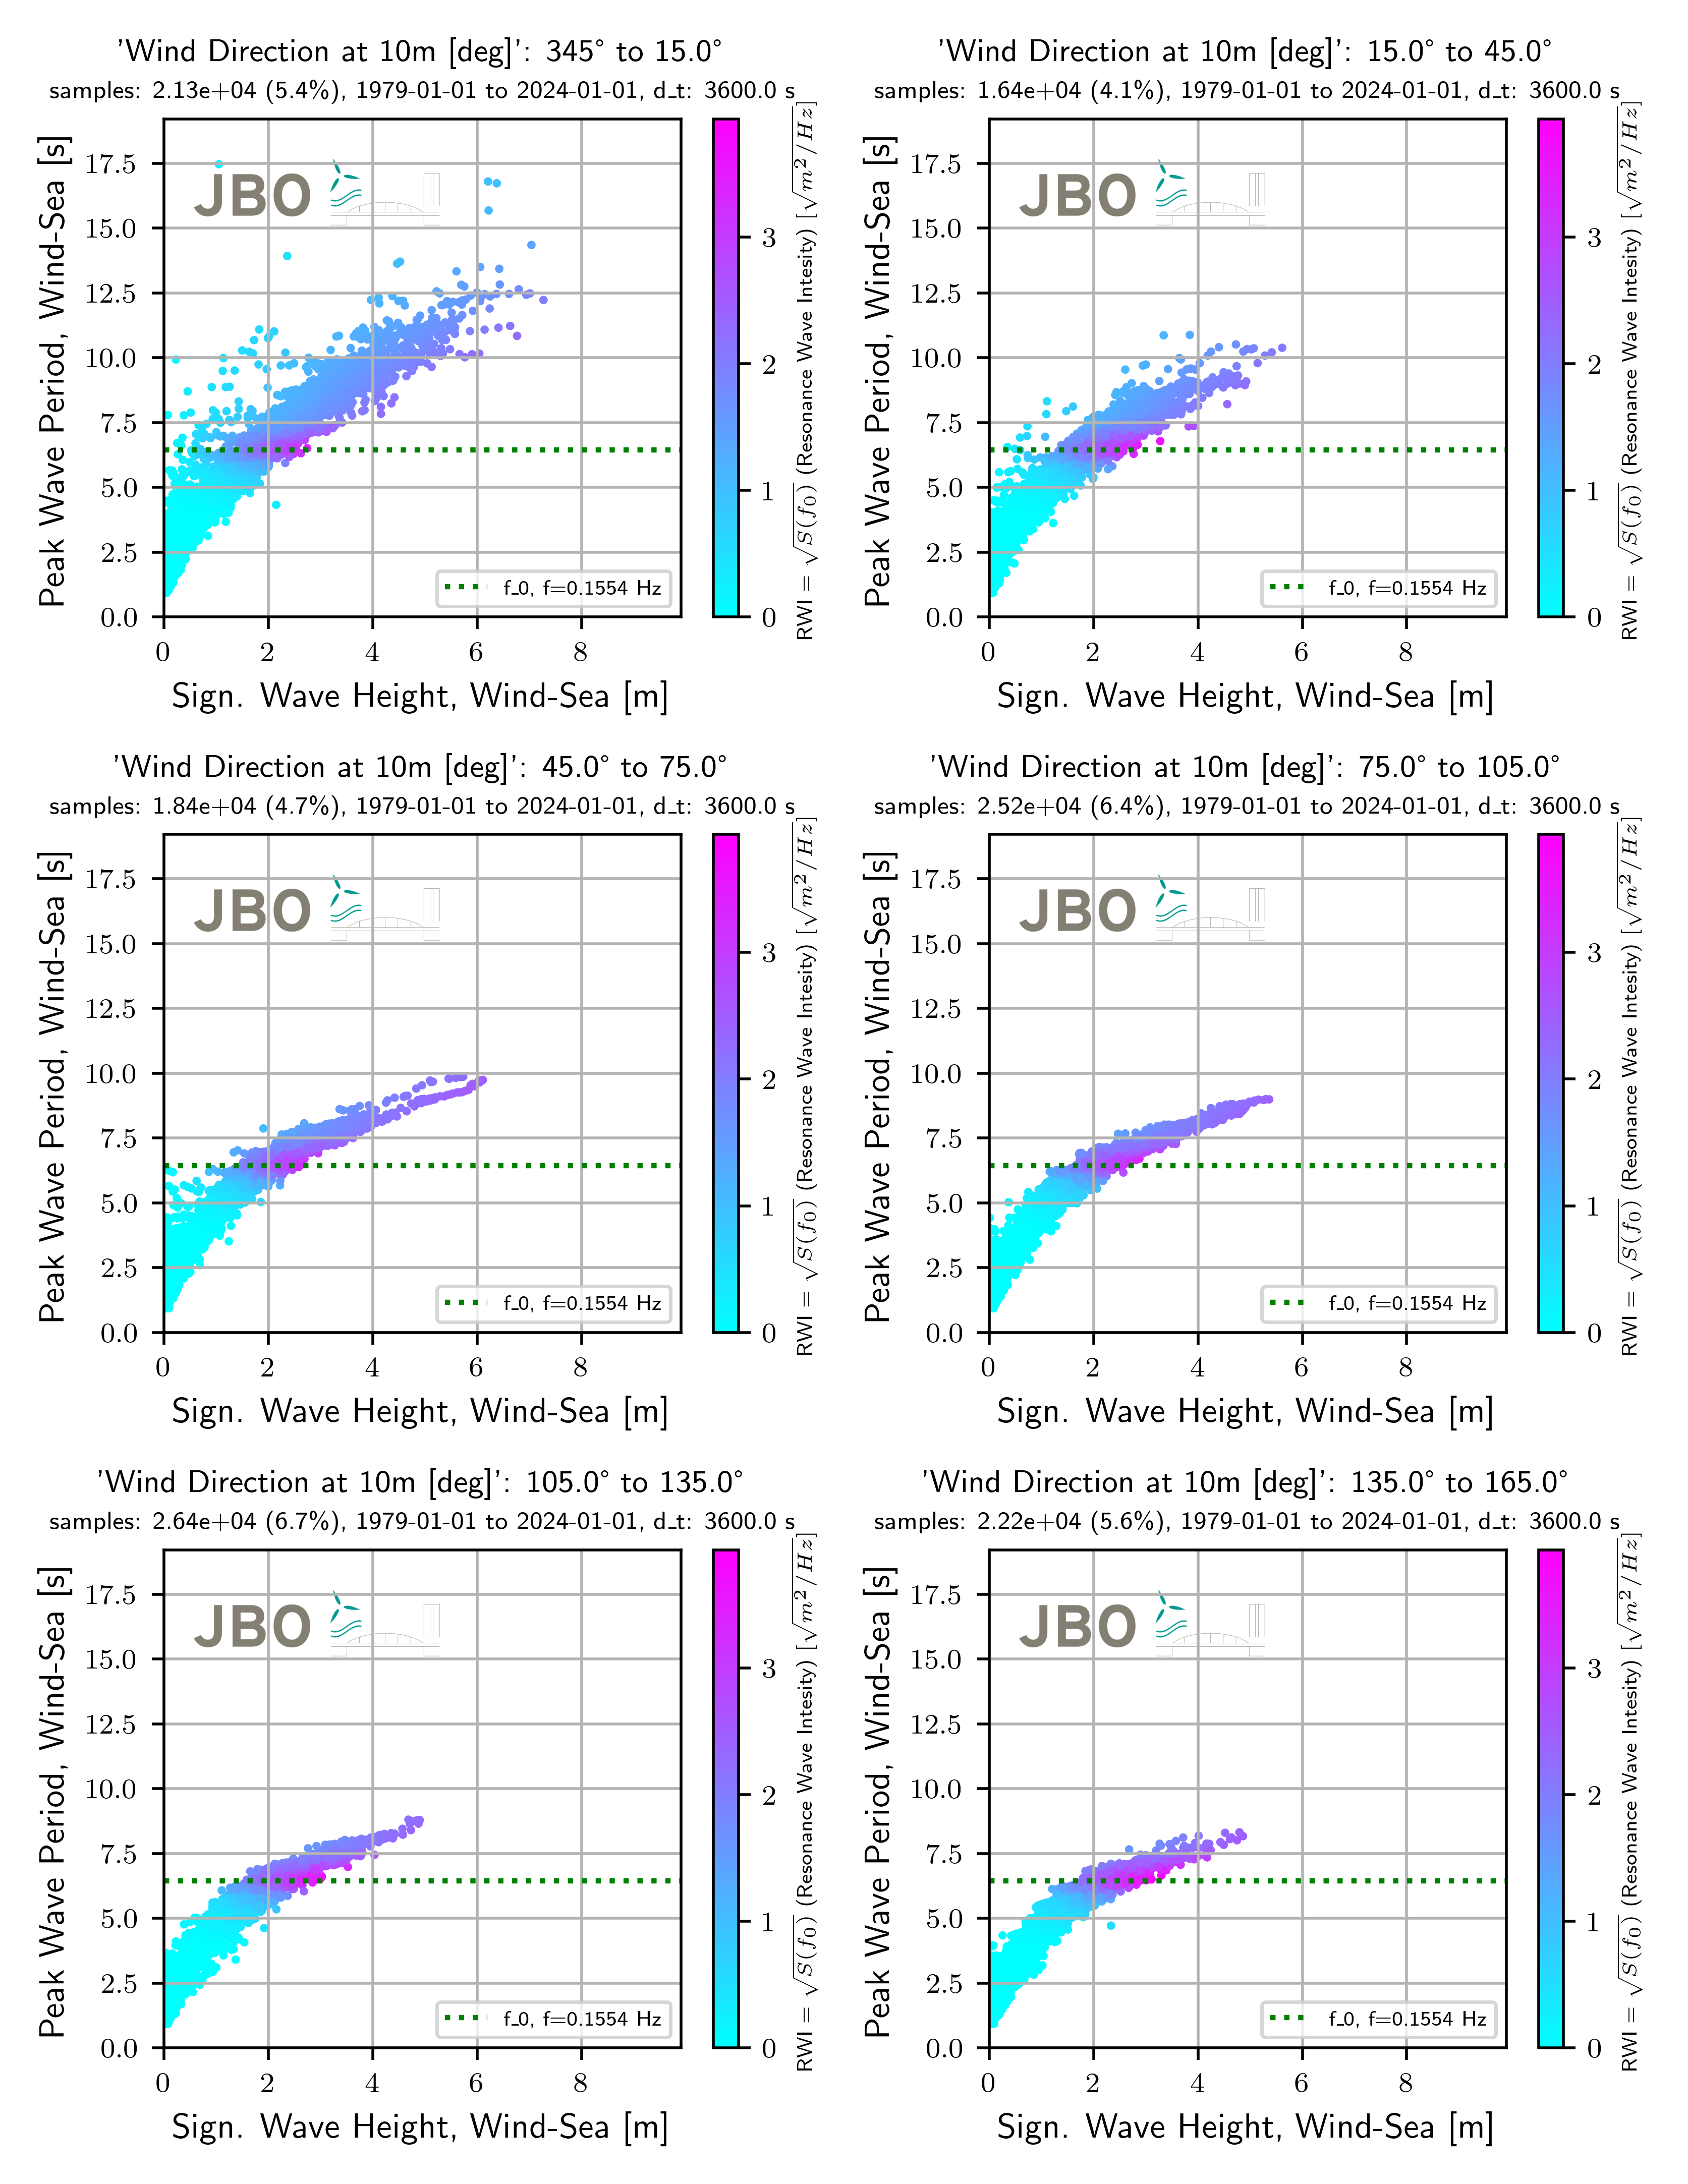
\includegraphics[width=1.0\textwidth]{C:/Users/aaron.lange/Desktop/Projekte/Hindcast_Tool/HindTool/example_output/RWI_wind_page_1.png} 
 \caption{ RWI-wind-page-1 } 
 \label{fig: RWI_wind_page_1 } 
\end{figure}
\begin{figure}[H] 
 \centering 
 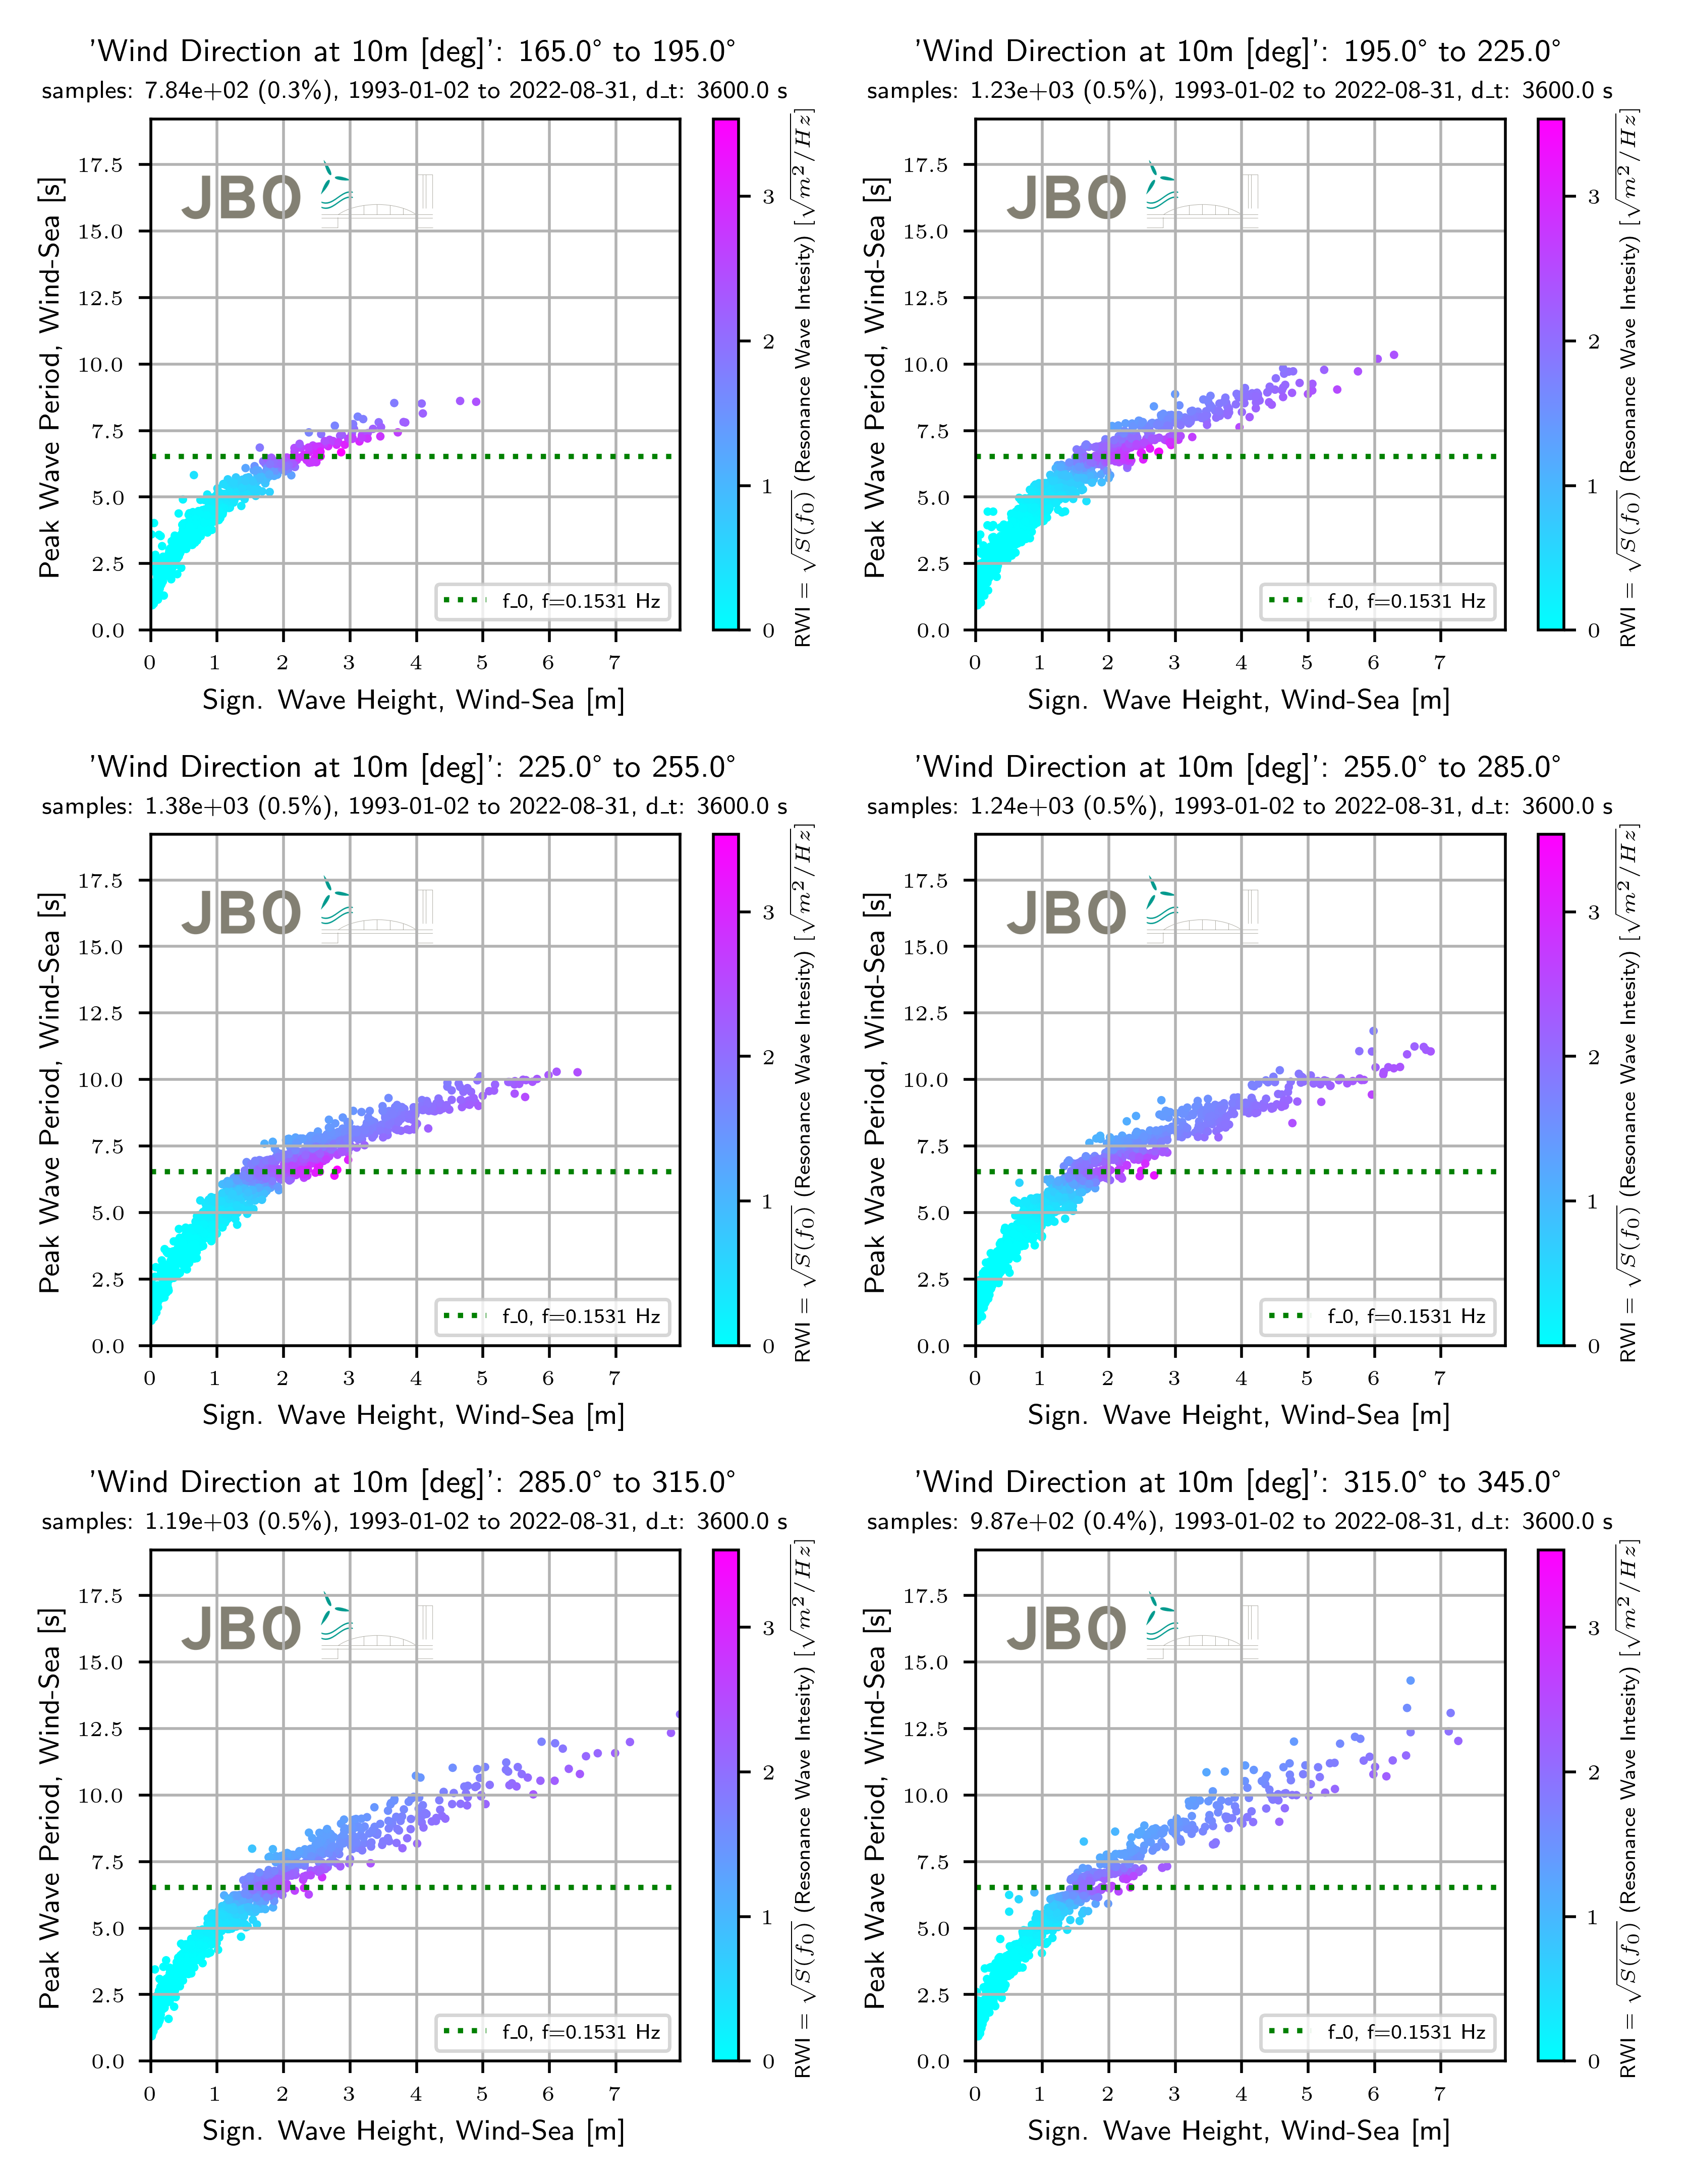
\includegraphics[width=1.0\textwidth]{C:/Users/aaron.lange/Desktop/Projekte/Hindcast_Tool/HindTool/example_output/RWI_wind_page_2.png} 
 \caption{ RWI-wind-page-2 } 
 \label{fig: RWI_wind_page_2 } 
\end{figure}
